\documentclass[]{article}
\usepackage{lmodern}
\usepackage{amssymb,amsmath}
\usepackage{ifxetex,ifluatex}
\usepackage{fixltx2e} % provides \textsubscript
\ifnum 0\ifxetex 1\fi\ifluatex 1\fi=0 % if pdftex
  \usepackage[T1]{fontenc}
  \usepackage[utf8]{inputenc}
\else % if luatex or xelatex
  \ifxetex
    \usepackage{mathspec}
  \else
    \usepackage{fontspec}
  \fi
  \defaultfontfeatures{Ligatures=TeX,Scale=MatchLowercase}
\fi
% use upquote if available, for straight quotes in verbatim environments
\IfFileExists{upquote.sty}{\usepackage{upquote}}{}
% use microtype if available
\IfFileExists{microtype.sty}{%
\usepackage{microtype}
\UseMicrotypeSet[protrusion]{basicmath} % disable protrusion for tt fonts
}{}
\usepackage[margin=1in]{geometry}
\usepackage{hyperref}
\hypersetup{unicode=true,
            pdftitle={Untitled},
            pdfauthor={Daniel Hsiao},
            pdfborder={0 0 0},
            breaklinks=true}
\urlstyle{same}  % don't use monospace font for urls
\usepackage{graphicx,grffile}
\makeatletter
\def\maxwidth{\ifdim\Gin@nat@width>\linewidth\linewidth\else\Gin@nat@width\fi}
\def\maxheight{\ifdim\Gin@nat@height>\textheight\textheight\else\Gin@nat@height\fi}
\makeatother
% Scale images if necessary, so that they will not overflow the page
% margins by default, and it is still possible to overwrite the defaults
% using explicit options in \includegraphics[width, height, ...]{}
\setkeys{Gin}{width=\maxwidth,height=\maxheight,keepaspectratio}
\IfFileExists{parskip.sty}{%
\usepackage{parskip}
}{% else
\setlength{\parindent}{0pt}
\setlength{\parskip}{6pt plus 2pt minus 1pt}
}
\setlength{\emergencystretch}{3em}  % prevent overfull lines
\providecommand{\tightlist}{%
  \setlength{\itemsep}{0pt}\setlength{\parskip}{0pt}}
\setcounter{secnumdepth}{5}
% Redefines (sub)paragraphs to behave more like sections
\ifx\paragraph\undefined\else
\let\oldparagraph\paragraph
\renewcommand{\paragraph}[1]{\oldparagraph{#1}\mbox{}}
\fi
\ifx\subparagraph\undefined\else
\let\oldsubparagraph\subparagraph
\renewcommand{\subparagraph}[1]{\oldsubparagraph{#1}\mbox{}}
\fi

%%% Use protect on footnotes to avoid problems with footnotes in titles
\let\rmarkdownfootnote\footnote%
\def\footnote{\protect\rmarkdownfootnote}

%%% Change title format to be more compact
\usepackage{titling}

% Create subtitle command for use in maketitle
\newcommand{\subtitle}[1]{
  \posttitle{
    \begin{center}\large#1\end{center}
    }
}

\setlength{\droptitle}{-2em}
  \title{Untitled}
  \pretitle{\vspace{\droptitle}\centering\huge}
  \posttitle{\par}
  \author{Daniel Hsiao}
  \preauthor{\centering\large\emph}
  \postauthor{\par}
  \predate{\centering\large\emph}
  \postdate{\par}
  \date{November 12, 2018}

\usepackage{placeins}

\begin{document}
\maketitle

{
\setcounter{tocdepth}{3}
\tableofcontents
}
\newpage

\hypertarget{methodology}{%
\section{Methodology}\label{methodology}}

\hypertarget{standard-approach}{%
\subsection{Standard Approach}\label{standard-approach}}

Consider the two variable case here for illustration purpose. The
multivariate case is provided in the appendix for completeness. We have
two forecasts, \(y_1\) and \(y_2\), of the true variable \(y\). We want
to combine \(y_1\) and \(y_2\) with a weight \(w\) that we have
\(y_c = w y_1 + (1-w) y_2\). Assume they follow some distribution, e.g.
\(y_1 \sim D(0,\sigma_1)\), \(y_2 \sim D(0,\sigma_2)\), and
\(corr(y_1,y_2)=\rho\). Then the variance of the combined forecast
\(y_c\) is \begin{equation}
\label{eqn: var yc}
Var(y_c) = w^2\sigma_1^2+ (1-w)^2\sigma_2^2+2w(1-w)\sigma_1\sigma_2\rho,
\end{equation} and the optimal weight with minimal variance is
\begin{equation}
\label{eqn: simple weight}
w^*=\frac{\sigma_2^2-\sigma_1\sigma_2\rho}{\sigma_1^2+\sigma_2^2 -2\sigma_1\sigma_2\rho}.
\end{equation}

Equation \ref{eqn: simple weight} is the standard benchmark approach in
the combination theory, where extensive research had been done on.
\textbf{add research}. Equation \ref{eqn: simple weight} has a few
empirical results that are against this approach. Two common
alternatives are diagonal covariance matrix and equal weights.

Ignoring the correlation term \(\rho\) by setting \(\rho=0\), we get the
inverse relation on the variance \begin{equation}
\label{eqn: simple weight no corr}
w^*=\frac{\sigma_2^2}{\sigma_1^2+\sigma_2^2}.
\end{equation} This is a robust way to avoid the estimation of the
covariance when the dimension goes up. The amount of parameter to
estimate for the covariance with dimension \(n\) is
\(\frac{1}{2}n(n+1)\), which is quadratic in \(n\). When the user only
estimates the variances, the amount of parameter to estimate reduces to
\(n\), which greatly decreases the estimation error. \textbf{add
citation}

Equal weights is another common approach that works better empirically.
\textbf{add citation} The forecast combination is in this case just an
arithmetric mean of all forecasts. The reason behind this is the fact
that estimating weights increases or shifts the forecast errors due to
additional estimation error in the estimation of \(w\). We laborate on
the estimation error of \(w\) more later.

\textbf{add more on equal weight}

\hypertarget{with-estimation-error-of-w}{%
\subsection{\texorpdfstring{With estimation error of
\(w\)}{With estimation error of w}}\label{with-estimation-error-of-w}}

We can also consider the weight as non-deterministic, but related with
\(y\), e.g., in a trivairate distribution with finite third and fourth
moments. Under trivariate distribution, the variance of the weights
influences the expected value and the variance of the combined forecast.
The expected value and the variance of the combined forecast becomes
\begin{equation}
\label{eqn: E & var yc w/ var w}
\begin{aligned}
  E(y_c) =& \mu + (cov(w, y_1-y_2))^2\\
var(y_c) =& E(w)^2\sigma_1^2 + (1-E(w))^2\sigma_2^2 + 2E(w)(1-E(w))\rho\sigma_1\sigma_2 \\
+& E[(w-E(w))(y_1-y_2) (E(w)y_1 + (1-E(w))y_2 - \mu)] \\
+& E[(w-E(w))^2 (y_1-y_2)^2] - cov(w,y_1-y_2)^2.
\end{aligned}
\end{equation}

Equation \ref{ eqn: E & var yc w/ var w} shows the general case of the
forecast combination. If the covariance between \(w\) and \(y_1-y_2\) is
not \(0\), the forecast is biased when combining, with bias
\(cov(w, y_1-y_2)^2\). The variance also increases from euqation
\ref{eqn: var yc} with
\(E[(w-E(w))(y_1-y_2) (E(w)y_1 + (1-E(w))y_2 - \mu)]+E[(w-E(w))^2 (y_1-y_2)^2] - cov(w,y_1-y_2)^2\).
\textbf{can we prove that the change in var(yc) is positive? I tried to
prove it but got stuck at
\(E[(w-E(w))(y_1-y_2) (E(w)y_1 + (1-E(w))y_2 - \mu)]+Var((w-Ew)(y_1-y_2))>0\)}.
This case the only requirements are that the individual forecast to be
unbaised and that the weights sum up to 1.

\hypertarget{truncation-approach}{%
\subsection{Truncation Approach}\label{truncation-approach}}

Looking back to equation \ref{eqn: simple weight}, we examin the effect
of high correlation term. Assume without loss of generality that
\(\sigma_1 =\sigma_2 + \delta\), where \(\delta>0\), we rewrite the
weight as \begin{equation}
\label{eqn: w high corr}
w = \frac{\sigma_2(-\rho\delta+ (1-\rho)\sigma_2)}{\sigma_1^2+\sigma_2^2 -2\sigma_1\sigma_2\rho}.
\end{equation} The numerator in \(w\) consist of standard deviation of
\(\sigma_2\) and a weighted mean between \(-\delta\) and \(\sigma_2\)
with weight \(\rho\). When \(\rho\) is small, the weights is close to
equation \ref{eqn: simple weight no corr}. When \(\rho\) is large, the
negative difference in variance \(-\delta\) takes over and results in
negative weights. The level of negativity accounts for both the negtaive
difference and correlation. The boundary case is \begin{equation}
\label{eqn: corr boundary}
\rho = \frac{\sigma_2}{\sigma_1},
\end{equation} which \(w\) decreases to \(0\) and \(y_c = y_2\). Figure

\begin{figure}[!h]
\centering
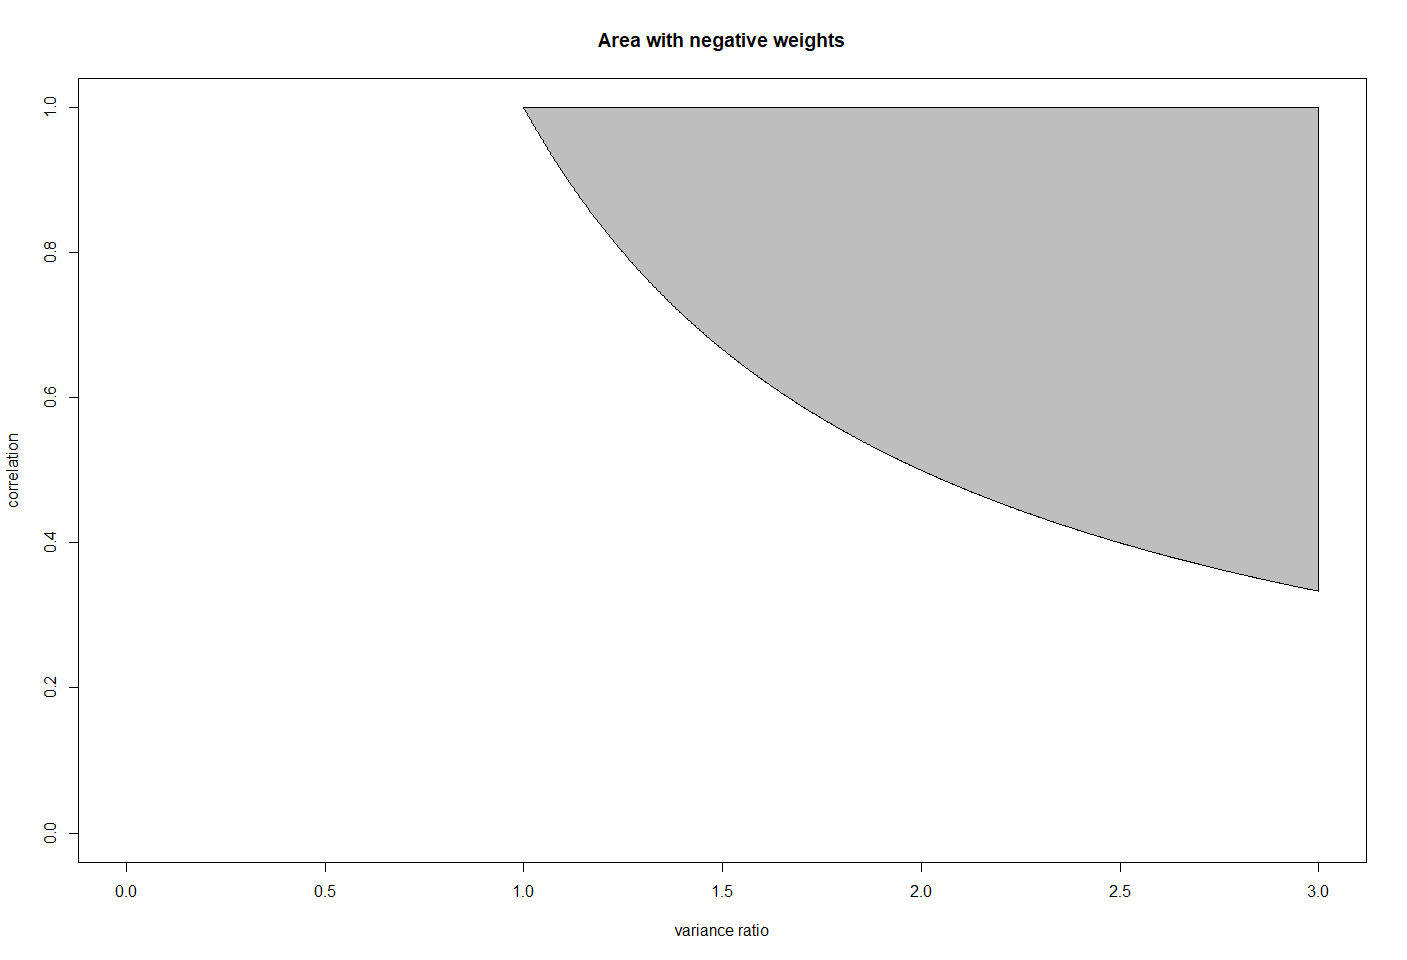
\includegraphics[width=8cm, height=8cm]{./Output/Images/corr2Ratio.png}
\caption{Plot of correlation and variance ratio. Grey area is where the weights become negative.}\label{fig: corr2Ratio}
\end{figure}

\hypertarget{bias-correction}{%
\subsection{Bias Correction}\label{bias-correction}}

\hypertarget{survey-of-professional-forecasters-spf}{%
\section{Survey of Professional Forecasters
(SPF)}\label{survey-of-professional-forecasters-spf}}

To illustrate the empirical results, we use the data from ECB
\textbf{(footnote link to data)} in this paper. The data, SPF, is a
quarterly survey initiated by ECB, with the aim to obtain future
estimates on inflation (HICP), RGDP and unemployment rate (UNEM) from
the private sector. Every quarter, a gourp of professional forecasters
from financial and non-financial instutition, such as economic research
institutions, respond to the survey with the idea on the future
economic. Starting 1999, SPF is the longest survey of macroeconomic
expectation in the euro area. Until the date of this paper, there are 75
quarters of observation available, with 1999 Q4 as the first forecasted
value, and 2018 Q2 as the last observed true macroeconomic indice.

The set up of the survey consist of multiple magnitudes of questions,
ranging from different horizon to different distribution. The
forecaststers are asked to provide their point forecast and the
probability of a certain scenario to happen. The survey enables ECB to
do quantitative assessment on the consensus of the market, like the
distribution statistics and standard deviations. For this paper, we take
the 2 most answered time periods, which is 1 year ahead and 2 year ahead
as our data set for all HICP, RGDP, and UNEM.

To compare the forecasts with the actual macroeconomics, we obtain the
true value from ECB data base \textbf{(footnote link to data)}. The data
cannot be observed from the economic in 100\% accuracy within the first
time frame, and exihibits changes to the initial estimates after
revision. We use the final estimate of the macroeconomics where
possible. The use of final estimate is fine is due to the fact that the
original forecast is not the real target to be forecasts.

Within the datasets, not all forecasters did a forecast every time
period. To avoid singular outliers, we remove all forecasters with a
total forecasted period of less than 24 quarter (6 years). The removal
approach is inline with \textbf{(ref paper)}.

Following \textbf{(ref paper)}, we calculate the covariance by looking
at the intersection between each forecasters.

\textbf{insert equation}

When there are no intersection between 2 forecasters, we set the
covariance value to 0. Additionally, we calculate the correlation by
using the covariance divided by the standard deviation. Standard
deviation is obtained from the square root of the diagonal.

\begin{equation}
\label{eqn: cov2cor}
\rho_{i,j} = \frac{\sigma_{i,j}}{\sigma_{i}\sigma_{j}}
\end{equation}

The cleaned up gives us a preliminary view on the SPF data without the
noises.

\begin{figure}[!h]
\centering
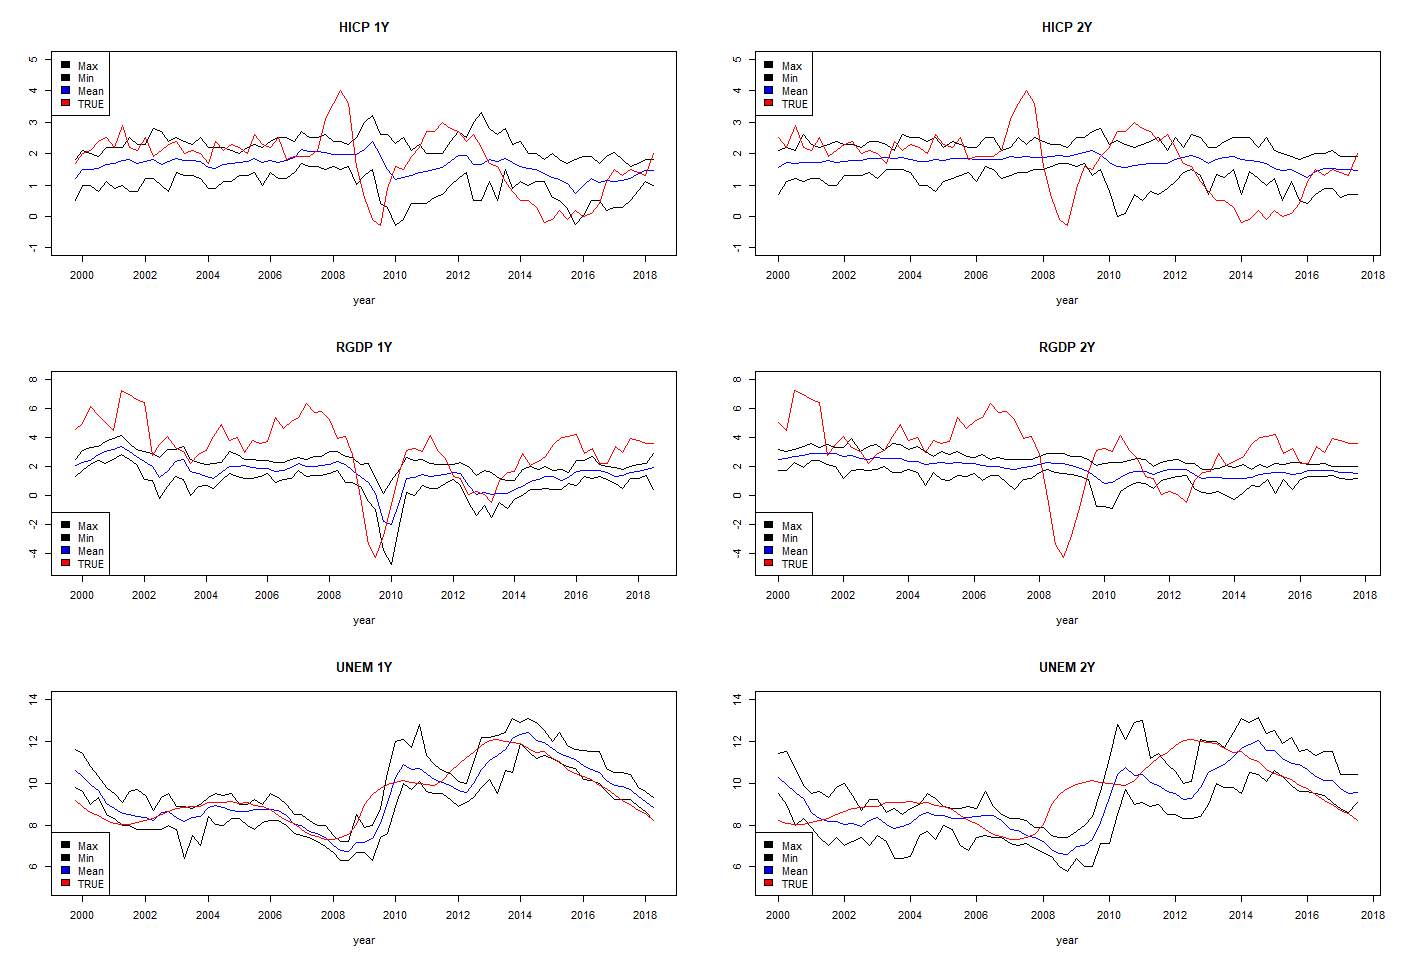
\includegraphics{./Output/Images/SPF.png}
\caption{Survey of Professional Forecasters data illustration}\label{fig: SPF data illustration}
\end{figure}

\textbackslash{}begin\{table\} \centering
\textbackslash{}caption\{Summary statistics of the correlation of the
forecast error. The correlation are split up into different forecast
topics and different forecast horizons. For all of the series, the
correlation are on average above 60\%. In HICP and UNEM the correlation
increases across all statistics when the forecast horizon increases,
while RGDP remains the same.\}
\label{tab: correlation summary statistics}

\begin{tabular}{lllllll}
\hline
Macro topic & \multicolumn{2}{c}{HICP} & \multicolumn{2}{c}{RGDP} & \multicolumn{2}{c}{UNEM} \\
Horizon     & 1 year & 2 year & 1 year & 2 year & 1 year & 2 year \\ \hline
min         & 0.03        & 0.02        & 0.11        & 0.13        & -0.02        & 0.08       \\
1st Q       & 0.53        & 0.62        & 0.63        & 0.65        & 0.47         & 0.56       \\
median      & 0.66        & 0.72        & 0.81        & 0.8         & 0.62         & 0.7        \\
mean        & 0.64        & 0.7         & 0.75        & 0.75        & 0.59         & 0.67       \\
3rd Q       & 0.77        & 0.81        & 0.89        & 0.87        & 0.74         & 0.8        \\
max         & 0.96        & 0.97        & 0.98        & 0.98        & 0.94         & 0.95       \\ 
\hline
\end{tabular}

\textbackslash{}end\{table\}

In figure \ref{fig: SPF data illustration} and table
\ref{tab: correlation summary statistics} we show the plots of the
forecasts along side with the true value in the macroeconomics and the
statistics of the covariance of the forecast error. To avoid too many
lines on the figure by plotting all forecasts, we plot only the minimum,
mean, and maximum from the forecasts. We see that there exist a high
consistency across all forecasts, with two years ahead stronger than one
year. The consistency in the forecast is lower in UNEM than the other
two. Furthermore, many true values lies outside of the forecast range,
with RGDP the worse of all three. More values outside of the forecast
range suggest that restricting positive weights may be a strong
limitation in the forecast combination. We expect to have large effect
using truncation in the forecast of RGDP, while HICP and UNEM does not
have too strong effect. We also expect the two year ahead forecast will
be better than the one year ahead.

The table \ref{tab: correlation summary statistics} tell us on how the
forecast error are correlated. The correlation are split up into
different forecast topics and different forecast horizons. Diagonal
element of the correlation matrix is not within the correlation when
generating the summary statistics. For all of the series, the
correlations are on average above 60\%. In HICP and UNEM the correlation
increases across all statistics when the forecast horizon increases,
while RGDP remains the same. The lowest correlation to be found is
-0.02, but this number is not too different than the minimum correlation
in the other two topics.

\textbf{add more explanation}

\hypertarget{empirical-results}{%
\section{Empirical Results}\label{empirical-results}}


\end{document}
